
\subsection{The Partition Coefficient}

This analysis investigated the peak dose rate contribution from various 
radionuclides to the partition coefficient of those radionuclides. 

The partition or distribution coefficient, $K_d$, relates the amount of contaminant adsorbed into the 
solid phase of the host medium to the amount of contaminant adsorbed into the 
aqueous phase of the host medium. It is a common empirical coefficient used to 
capture the effects of a number of retardation mechanisms. The coefficient 
$K_d$, in units of $[m^3\cdot kg^{-1}]$, is the ratio of the mass of contaminant in the 
solid to the mass of contaminant in the solution.

The parameters in this model were all set to the default values except a multiplier 
applied to the partitioning $K_d$ coefficients. The multiplier took the forty values $1\times10^{-9}, 5\times10^{-8}, \cdots 
5\times10^{10}$ Only the far field partition coefficients were altered by this 
factor. Partition coefficients effecting the EDZ and fast pathway were not 
changed.

The expected inverse relationship between the partition coefficient resulting 
peak annual dose was found for all elements that were not assumed to be 
effectively infinitely soluble.  It is clear from Figure \ref{fig:KdSum} that 
for partition coefficients greater than a threshold, the relationship between 
peak annual dose and partition coefficient is a strong inverse one. 

\begin{figure}[ht]
  \centering
  \includegraphics[width=\linewidth]{Partitioning_Summary.eps}
  \caption{$K_d$ sensitivity.  The peak annual dose due to an inventory, 
  $N$, of each isotope.}
  \label{fig:KdSum}
\end{figure}

